\subsection{Scénarios et chronologies de vol}
\label{subsec:scenarios_chronologies}

Un vol de fusée bi-étage actif, respectant le \acrshort{CDC} du \acrshort{CNES} et de \gls{Planète Sciences}, se différentie de celui d'une fusée classique.
En effet, beaucoup d'évenement en vol doivent se réaliser et le résultat de ces évenements influent sur la trajectoire de la fusée. Cette partie présente
les différents scénarios pris en compte par le logiciel de vol et la chronologie des évenements du vol.

\subsubsection{Présentation des scénarios}

Deux des évenement du vol influe particulièrement le profile de vol de la mission : \\

\hspace*{-\parindent}%
\begin{minipage}{0.5\textwidth}
    \begin{itemize}
        \item \textbf{Séparation} : Le système de séparation des deux étages de la fusée est considéré comme un système expérimental. Son bon foncionnement
        n'est donc pas un élément certain. Le non délpoiement de ce dernier correspond au scénario \texttt{SCE2}.
        \item \textbf{Allumage 2e étage} : L'allumage du moteur du deuxième étage est également un système expérimental. De plus, pour des raisons de
        sécurité, cet allumage ne doit être effectué que si la trajectoire courante respecte un certain gabarie. On distinguera alors deux sous-cas :
        \begin{itemize}
            \item La trajectoire ne respecte pas la plage de sécurité (scénario \texttt{SCE1.1})
            \item Le système d'allumage n'a pas fonctionné (scénario \texttt{SCE1.2})
        \end{itemize}
        Ces deux scénarios font partie du même scénario \texttt{SCE1} qui décrit le non allumage du moteur du deuxième étage.
    \end{itemize}
\end{minipage}
\hfill
\begin{minipage}{0.45\textwidth}
    \centering
    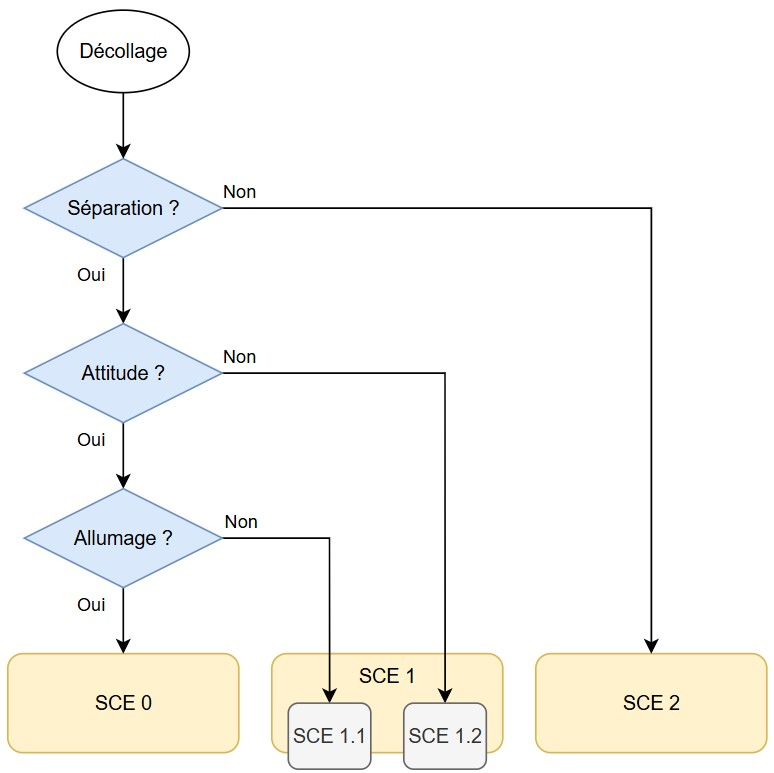
\includegraphics[width=\textwidth]{figures/SCE.jpg}
    \captionof{figure}{Différent scénarios}
    \label{fig:sces}
\end{minipage}

\subsubsection{Note de lecture des chronogrammes}

La convention de lecture de ces chronogrammes repose sur trois niveaux d'information. Le premier est la fenêtre temporelle,
identifiée par le préfixe "\texttt{FT\_}" et représentée par une zone hachurée : elle désigne l'intervalle à l'intérieur duquel
un événement donné (détection de séparation, d'allumage, d'apogée, ...) doit avoir lieu. Pendant toute cette plage, la logique
du lanceur exploite ses mesures et attend que l'ensemble des conditions propres à cet événement se réunissent pour que celui-ci
puisse survenir. Ce sont donc ces conditions, et non une date programmée, qui déterminent si l'événement a lieu et à quel moment.
Une fenêtre qui s'écoule sans que la convergence soit atteinte se traduit par un événement qui ne survient pas. L'instant réel de
déclenchement ne peut par conséquent pas être connu à l'avance. Le deuxième niveau, l'événement lui-même, matérialisé par un
losange, est donc placé à un instant temporel purement théorique choisi dans la fenêtre dans le seul but de rendre la séquence
lisible. Le troisième niveau regroupe les actions qui découlent de ces événements (commande d'actionneur, phase de combustion,
...), représentées par des barres pleines : leur durée est bien celle de l'action, mais leur position sur l'axe des temps est
ancrée sur l'horodatage théorique de l'événement déclencheur dont elles héritent.\\

Ces chronogrammes se lisent ainsi comme un enchaînement logique de conditions, d'événements et de conséquences, dans lequel
seuls l'ordonnancement des étapes et l'amplitude des fenêtres font foi. La convention étant appliquée de façon homogène aux
trois scénarios (\texttt{SCE\_0}, \texttt{SCE\_1}, \texttt{SCE\_2}), leur comparaison directe reste pertinente.

\newpage

\subsubsection{\texttt{SCE 2} : Vol sans séparation}

Ce scénario correspond au cas où la séparation des deux étages n'intervient pas. C'est le cas de figure le plus simple : le
lanceur se comporte de bout en bout comme un corps unique.

\begin{figure}[H]
    \centering
    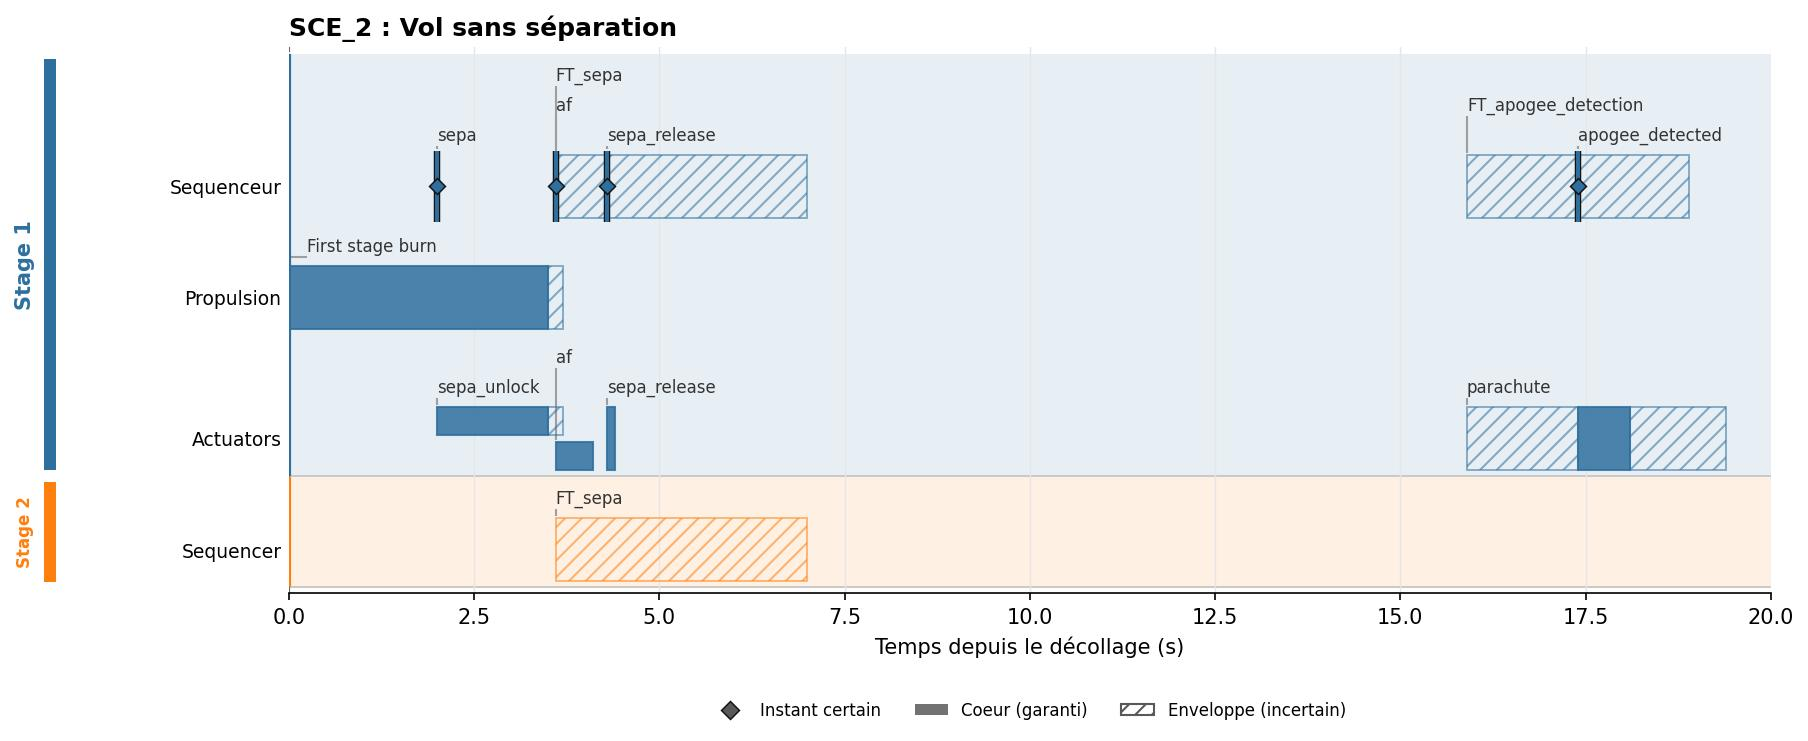
\includegraphics[width=\textwidth]{figures/timeline_sce2.jpg}
    \caption{Chronologie du scénario 2}
    \label{fig:timeline_sce2}
\end{figure}

La séquence se lit comme suit :

\begin{itemize}
    \item \textbf{$t = 0$~s — Décollage.} La combustion occupe la ligne \texttt{Propulsion} jusqu'à environ 3,5~s ; la courte
    extension hachurée jusqu'à 3,5~s traduit la dispersion attendue sur l'instant d'extinction.\\

    \item \textbf{$t = 2{,}0$~s — \texttt{sepa\_unlock}.} Commande de déverrouillage du mécanisme de séparation. Elle est
    émise en pleine phase propulsée et non après l'extinction afin d'absorber le délai qui sépare la commande de son effet : la
    ligne \texttt{Actionneurs} montre que le déverrouillage n'est effectivement acquis que vers 3,6~s soit après l'extinction du
    moteur du premier étage.\\

    \item \textbf{$t = 3{,}5$~s — Fin de combustion du premier étage.}\\

    \item \textbf{$t = 3{,}6$~s — \texttt{airbreakes}.} Déploiement des aérofreins, dont l'action s'achève vers 4,1~s. Au
    début du déploiement, les étages se comportent déjà comme deux corps distincts.\\  

    \item \textbf{$t = 3{,}6$~s à $7,0~s$ — \texttt{FT\_sepa}.} Fenêtre de détection de la séparation, ouverte simultanément
    sur les deux étages.\\

    \item \textbf{$t = 4{,}3$~s — \texttt{sepa\_release}.} Ordre de séparation par ressort.\\

    \item \textbf{$t = 7{,}0$~s — \texttt{FT\_sepa}.} Fermeture de la fenêtre de détection de la séparation. L'événement
    \texttt{sepa\_detected} n'est jamais déclaré, ce qui signifie que la séparation n'a pas été constatée par les étages. Le
    second étage ne démarre donc jamais sa propre séquence.\\

    \item \textbf{$t = 15{,}9$~s à $19,0$~s — \texttt{FT\_apogee\_detection}.} Fenêtre à l'intérieur de laquelle l'apogée
    doit être constaté.\\

    \item \textbf{$t = 17{,}4$~s — \texttt{apogee\_detected}.} L'apogée est déclaré, ce qui entraîne la mise en \oe uvre de
    la récupération. Si la fenêtre s'était écoulée sans que l'apogée ne soit constaté, la récupération aurait tout de même été
    déclenchée.
\end{itemize}

\newpage

\subsubsection{\texttt{SCE 1} : Vol avec séparation sans allumage du 2e étage}

Ce scénario reprend le déroulement de \texttt{SCE\_2} jusqu'à la séparation, qui cette fois est effectivement constatée. Le vol
se scinde alors en deux chronologies indépendantes. Cependant le moteur du second étage ne s'est jamais allumé.

\subsubsubsection{\texttt{SCE 1.2} : Attitude non conforme}

\begin{figure}[H]
    \centering
    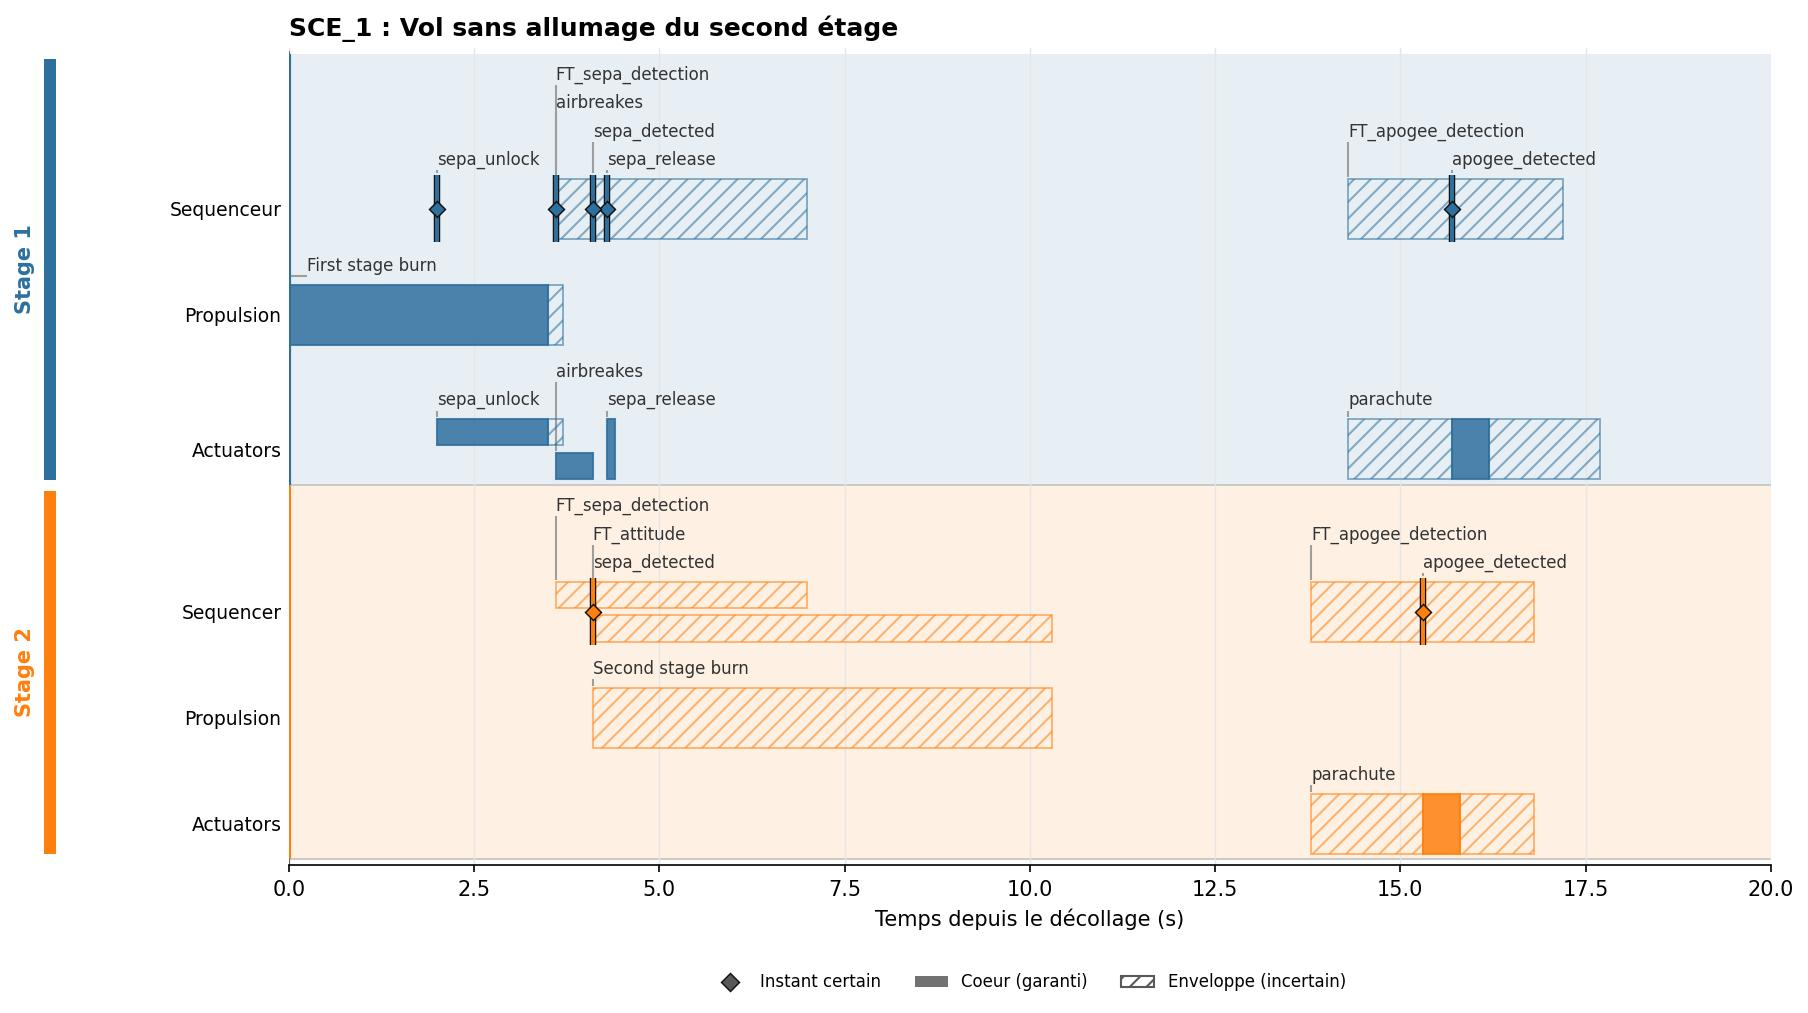
\includegraphics[width=\textwidth]{figures/timeline_sce1_2.jpg}
    \caption{Chronologie du scénario 1.2}
    \label{fig:timeline_sce1}
\end{figure}

Le déroulement de l'étage inférieur jusqu'au largage est identique à celui décrit en section~\ref{sec:sce2} et n'est pas repris
ici. Les éléments nouveaux ou modifiés sont les suivants :

\begin{itemize}
    \item \textbf{$t = 4{,}1$~s — \texttt{sepa\_detected}.} Au sein des fenêtres \texttt{FT\_sepa\_detection}, les séquenceurs
    ont constaté la séparation des deux étages. Le second étage démarre sa propre séquence : le chronogramme se lit désormais
    sur deux chronologies indépendantes.\\

    \item \textbf{$t = 3{,}9$~s à $10,3$~s — \texttt{FT\_attitude}.} Fenêtre pendant laquelle la logique du second étage
    surveille son orientation et sa stabilité, conditions préalables à l'autorisation d'allumage du propulseur.\\

    \item \textbf{Ligne Propulsion du second étage.} L'enveloppe de la combustion est représentée de $3,9$~s à $10,3$~s.
    La combustion est attendue dans cette fenêtre mais n'a jamais lieu.\\

    \item \textbf{$t = 13{,}8$~s à $16,7$~s — \texttt{FT\_apogee\_detection} (étage 2).} Le second étage dispose désormais de
    sa propre fenêtre de détection d'apogée, distincte de celle du premier. Chacun surveille sa propre trajectoire avec sa propre
    logique.\\

    \item \textbf{$t = 15{,}3$~s — \texttt{apogee\_detected} (étage 2).} L'apogée du second étage est constaté et la
    récupération est mise en \oe uvre.
\end{itemize}

Le point caractéristique de ce scénario tient dans la fenêtre \texttt{FT\_attitude} : ouverte dès la séparation constatée, elle
s'écoule sans qu'aucun ordre n'en sorte. La logique du second étage n'a pas vu se réunir les conditions d'attitude qui
conditionnent l'autorisation d'allumage, et l'ordre correspondant n'est donc jamais émis. Les deux corps poursuivent dès lors un
vol purement balistique, chacun sous la conduite de son propre séquenceur. Le premier étage suit une chronologie qu'il aurait
suivie à l'identique en vol nominal, son comportement ne dépendant plus du second une fois le largage effectué.

\newpage

\subsubsubsection{\texttt{SCE 1.1} : Pousée du 2e étage non mesurée}

Ce scénario prolonge le précédent d'un cran dans la chaîne de conditions : les conditions d'attitude sont cette fois réunies et
l'ordre d'allumage est bien émis, mais l'allumage lui-même n'est jamais confirmé.

\begin{figure}[H]
    \centering
    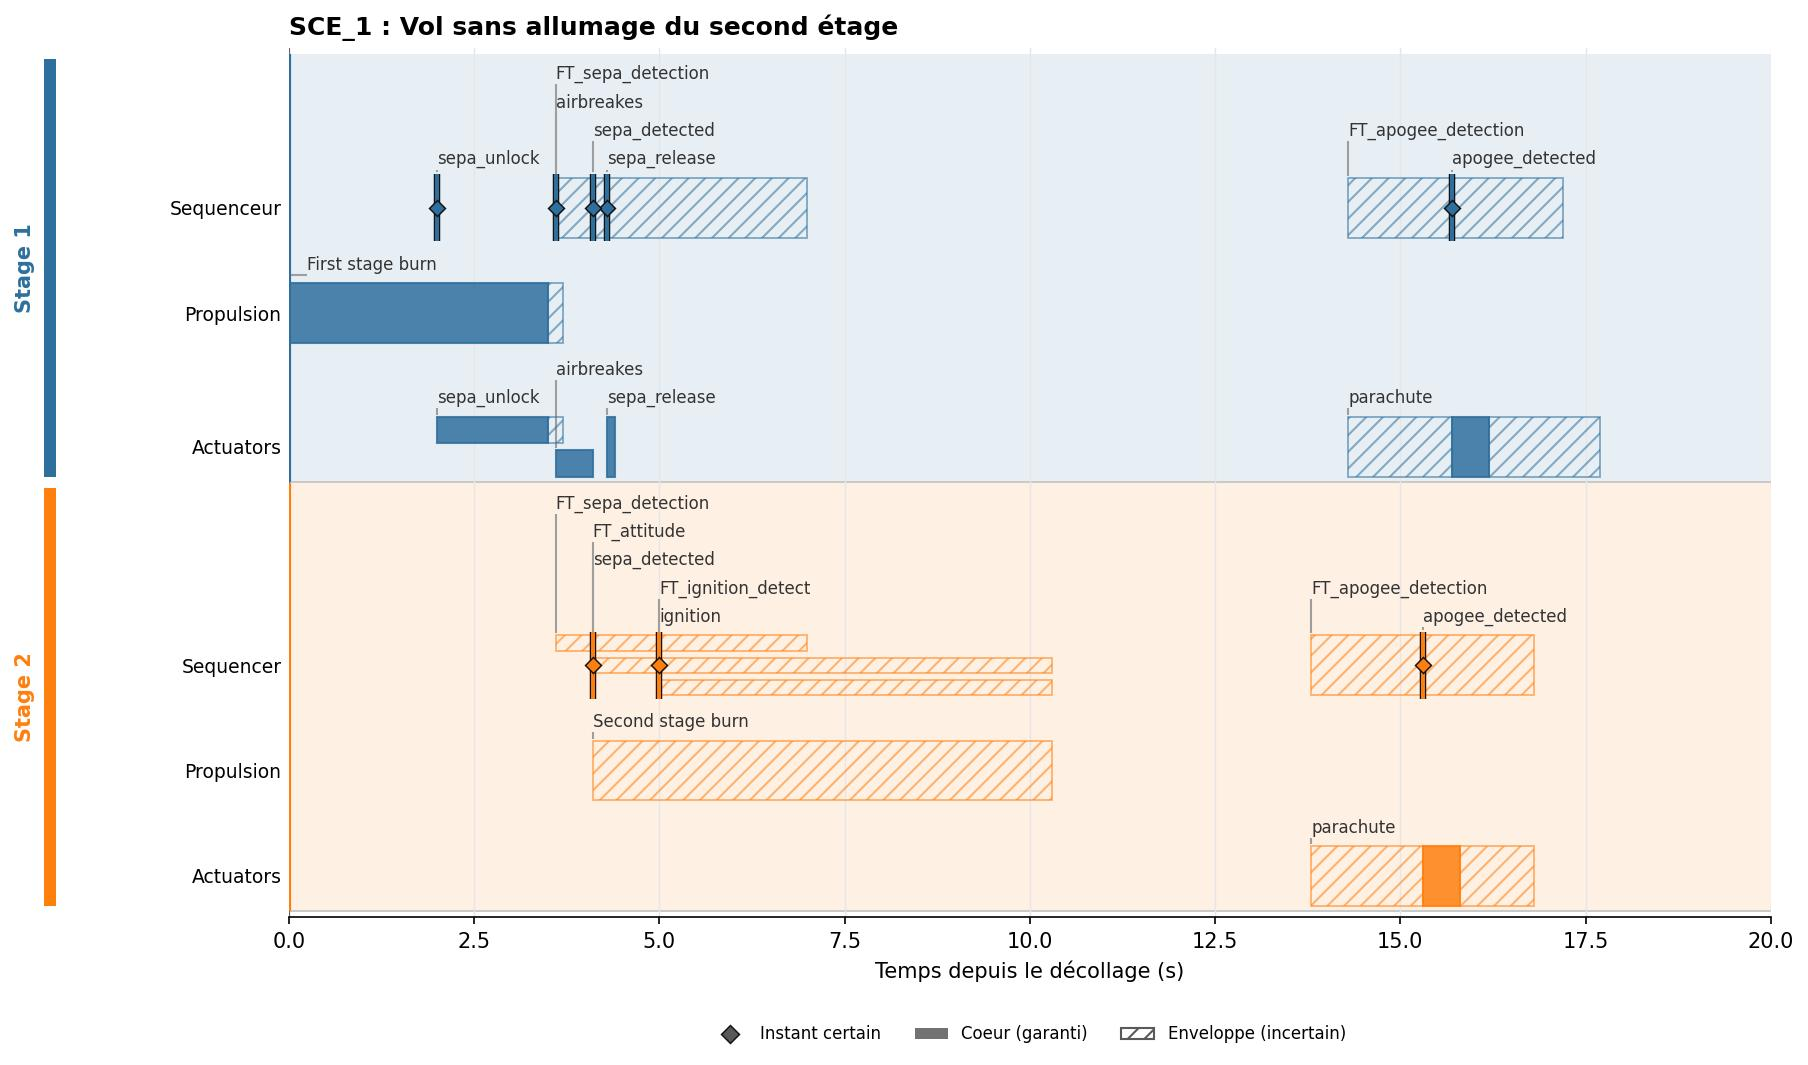
\includegraphics[width=\textwidth]{figures/timeline_sce1_1.jpg}
    \caption{Chronologie du scénario 1.1}
    \label{fig:timeline_sce1}
\end{figure}

Par rapport à SCE\_1.2 (section~\ref{sec:sce1-2}), deux éléments s'ajoutent :

\begin{itemize}
  \item \textbf{$t \approx 5{,}0$~s — \texttt{ignition}.} Ordre d'allumage, émis dès que les conditions surveillées dans
  \texttt{FT\_attitude} sont réunies.\\

  \item \textbf{$t \approx 5{,}0$~s à $10,3$~s — \texttt{FT\_ignition\_detect}.} Fenêtre à l'intérieur de laquelle la logique
  du second étage doit constater, à partir de ses mesures, que l'allumage a effectivement eu lieu.
\end{itemize}

L'ordre \texttt{ignition} et sa confirmation \texttt{ignition\_detected} sont deux événements de nature différente. Le premier
est émis par le séquenceur dès que ses conditions d'entrée sont satisfaites alors que le second est une constatation physique,
subordonnée au comportement de la chaine d'allumage réel et du moteur.\\

La suite du vol est en conséquence identique à celle de SCE\_1.2 : les deux étages poursuivent un vol balistique et exécutent
chacun leur séquence de récupération aux mêmes instants.

\newpage

\subsubsection{\texttt{SCE 0} : Vol avec séparation et allumage du 2e étage}

Ce scénario est celui du vol nominal : la chaîne de conditions est parcourue jusqu'à son terme, l'allumage du second étage est
confirmé et la combustion a lieu.

\begin{figure}[H]
    \centering
    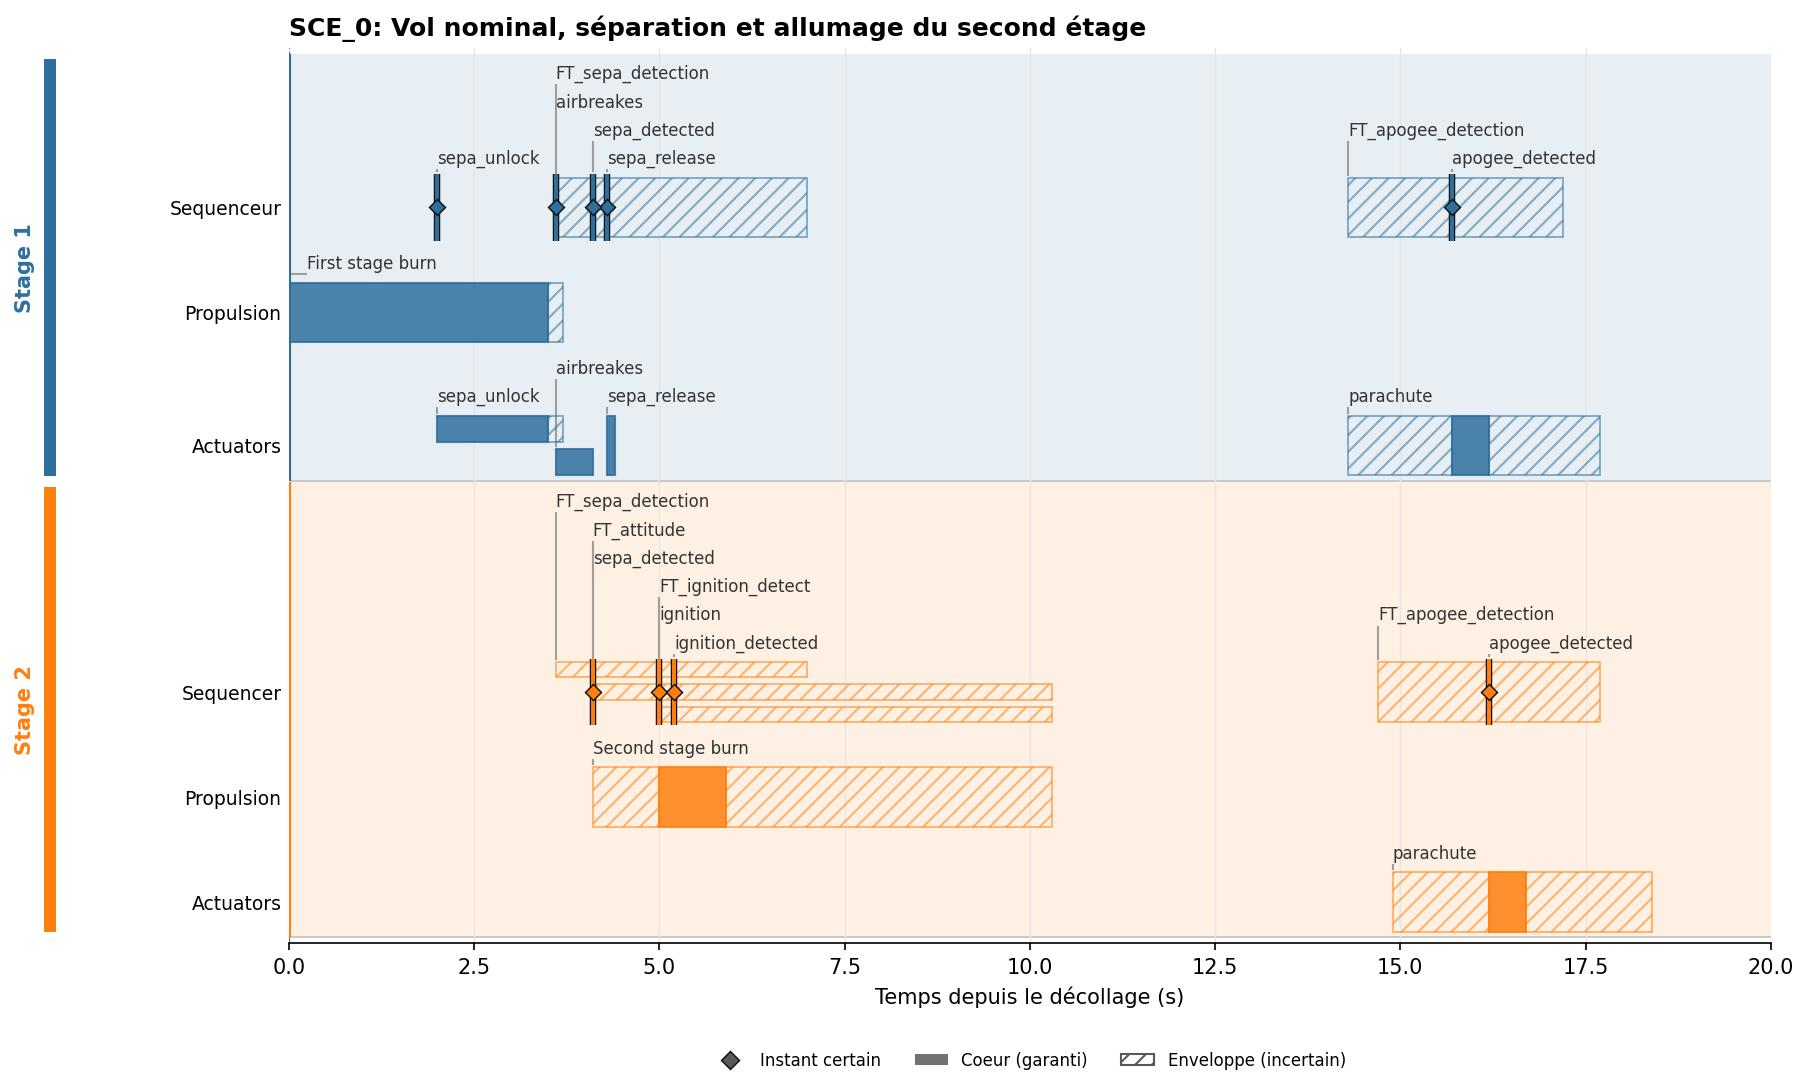
\includegraphics[width=\textwidth]{figures/timeline_sce0.jpg}
    \caption{Chronologie du scénario 0}
    \label{fig:timeline_sce0}
\end{figure}

Les éléments nouveaux sont les suivants :

\begin{itemize}
    \item \textbf{$t \approx 5{,}2$~s — \texttt{ignition\_detected}.} La confirmation attendue en vain dans \texttt{SCE\_1.1}
    est cette fois déclarée, à l'intérieur de la fenêtre \texttt{FT\_ignition\_detect}.

    \item \textbf{$t \approx 4{,}9$~s à $5,7$~s — combustion du second étage.} Un c \oe ur apparaît pour la première fois sur
    la ligne \texttt{Propulsion} du second étage, à l'intérieur de l'enveloppe déjà présente dans les scénarios précédents. La
    combustion, d'environ une seconde, constitue le seul apport d'énergie postérieur à la séparation.
\end{itemize}

Dans ce scénario, aucune fenêtre ne reste vide : séparation constatée, conditions d'attitude réunies, ordre d'allumage émis,
allumage confirmé, combustion effective.

\newpage

\subsubsection{Comparaison des instants d'apogée selon les scénarios}
\label{sec:apogees}

L'apogée constitue le point où les trajectoires des différents scénarios se distinguent le plus nettement, et il conditionne
directement la séquence de récupération. Les fenêtres \texttt{FT\_apogee\_detection} des trois scénarios sont donc regroupées
ici sur un même axe afin d'être comparées entre elles.

\begin{figure}[H]
    \centering
    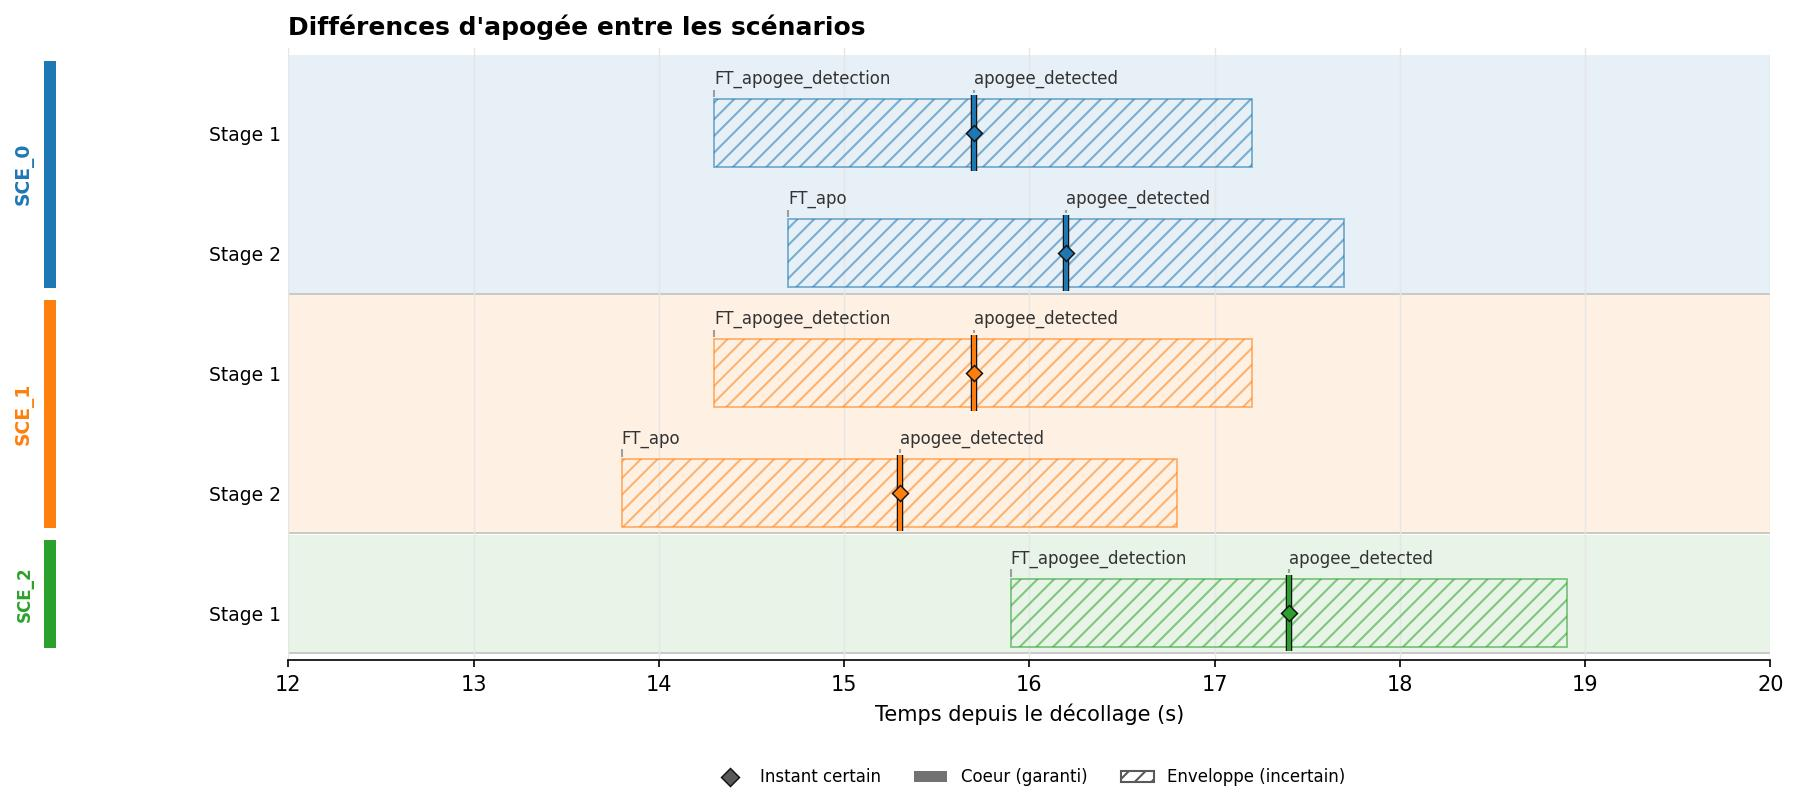
\includegraphics[width=\textwidth]{figures/timeline_sce_apo.jpg}
    \caption{Zoom sur la phase d'apogée des scénarios}
    \label{fig:timeline_sce_apo}
\end{figure}

Les scénarios SCE\_1.1 et SCE\_1.2 sont ici confondus sous l'appellation
SCE\_1 : aucune combustion n'ayant lieu dans l'un comme dans l'autre, leur
chronologie de récupération est rigoureusement identique. Le maillon de la
chaîne d'allumage sur lequel la séquence s'est interrompue n'a donc aucun effet
en aval.

\begin{table}[H]
    \centering
    \begin{tabular}{llcc}
        \toprule
        Scénario & Étage & \texttt{FT\_apogee\_detection} & \texttt{apogee\_detected} \\
        \midrule
        SCE\_0 & Étage 1 & 14,3 -- 17,2~s & 15,7~s \\
        SCE\_0 & Étage 2 & 14,7 -- 17,7~s & 16,2~s \\
        SCE\_1 & Étage 1 & 14,3 -- 17,2~s & 15,7~s \\
        SCE\_1 & Étage 2 & 13,8 -- 16,8~s & 15,3~s \\
        SCE\_2 & Ensemble & 15,9 -- 18,9~s & 17,4~s \\
        \bottomrule
    \end{tabular}
    \caption{Fenêtres de détection d'apogée et instants théoriques associés.}
    \label{tab:apogees}
\end{table}

On remarque un ordonnancement des apogées, qui s'explique selon l'énergie et la masse de chaque corps.\\
\begin{enumerate}
    \item L'ensemble non séparé de SCE\_2 culmine le plus tard : il conserve la masse totale et donc l'inertie la plus grande.
    Il décélère donc le moins.\\
    \item Le second étage de SCE\_0, seul corps à avoir reçu une impulsion après la séparation. Cependant, le propulseur utilisé
    pour la campagne de vol n'est pas très performant pour la masse du second étage.\\
    \item Le premier étage est l'étage seul suivant une trajectoire purement balistique le plus lourd.\\
    \item Enfin, le second étage non allumé de SCE\_1 culmine le plus tôt.
\end{enumerate}

\newpage
